\section{Experiments}

The objective of this experiment is to classify images into three hair types. To achieve this, we tested different hyperparameters, explored various preprocessing tecniques and experimented in creating the optimal CNN architecture. The primary goals in this experiment were to optimize evaluation metrics and minimize overfitting, ensuring robust model performance.

\subsection{Adjustment of Image Size and Batch Size}

The initial image size was set to \(64 \times 64\) pixels. While this smaller dimension allowed us to train the model faster, it compromised the quality of the training images, potentially eliminating important information for accurate classification. Conversely, increasing the image size to \(512 \times 512\) pixels significantly increased the training time to almost 30 minutes, which was impractical for our computational resources. Our experiments was conducted on a laptop with specifications of a GTX 1660Ti graphics card, a Ryzen 7 4800H processor, and 32GB of RAM.

Thambawita et al. (2021) \cite{smith2021edge} discussed in their paper that the performance of the classification model is dependent upon the resolution of images, but it is important to consider the trade-off between image size and the time needed for training the model. Considering these factors, we opted to use an image size of \(256 \times 256\) pixels. This resolution provides an optimal balance between image quality and manageable training times. 

\begin{figure}[H]
    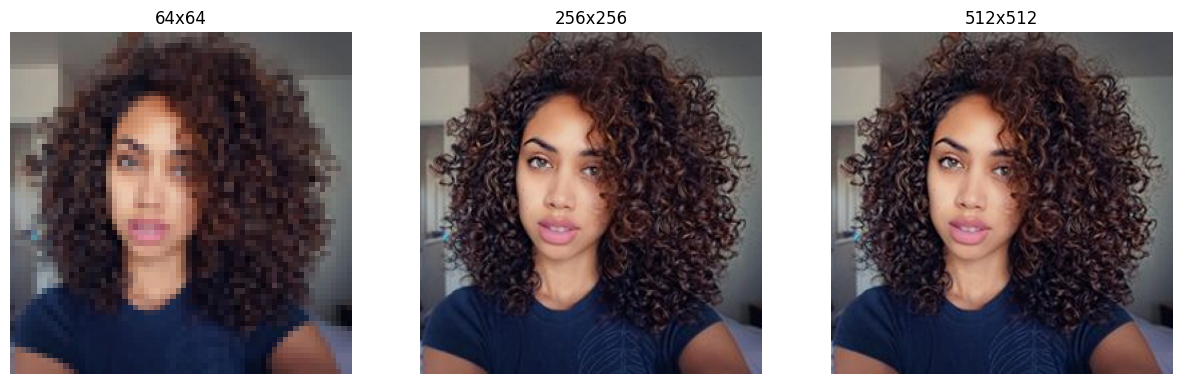
\includegraphics[width=\linewidth]{figures/image_sizes.png}
    \caption{Different Image Resolution}
    \label{fig:image_sizes}
  \end{figure}

Regarding the batch size, we experiments with sizes that are divisible by our image size, such as 32, 64, and 128. The batch size of 64 was chosen as it offers an efficient balance between minimizing the memory usage during training while providing a reliable estimate of the gradient. 

For the batch size, we used 64. We tested using batch size of 128 and 32 for this model since they are all divisible by 256 which is the image size, but we opted to continue using 64 for a better balance of requiring less memory in training and the accuracy of the estimate of the gradient.

\subsection{Preprocessing}

During the experimental phase, we utilized two preprocessing techniques in machine learning for image classification: Sobel Edge Detection and Data Augmentation. These methods were chosen based on their potential to improve model accuracy and minimize overfitting.

The models were evaluated under four different preprocessing scenarios to assess their impact:

\begin{itemize}
    \item No preprocessing
    \item With Sobel Edge Detection only
    \item With Data Augmentation only
    \item With both Sobel Edge Detection and Data Augmentation
\end{itemize}

\begin{table}[h]
\centering
\caption{Comparative Results of Different Preprocessing Techniques}
\label{tab:preprocessing_results}
\begin{tabular}{|l|c|c|p{5cm}|}
\hline
\textbf{Preprocessing Scenario} & \textbf{Training Accuracy} & \textbf{Validation Accuracy} & \textbf{Training Loss} & \textbf{Validation Loss} \\ \hline
No preprocessing & 0.6392 & 0.5431 & 0.7715 & 0.9983 \\ \hline
With Sobel Edge Detection only & 0.6145 & 0.5867 & 0.8398 & 1.0101 \\ \hline
With Data Augmentation only & 0.4311 & 0.5431  & 1.0880  & 0.9833 \\ \hline
With Sobel Edge Detection \& Augmentation & 0.4041 & 0.4112 & 1.1733 & 1.1114 \\ \hline
\end{tabular}
\end{table}

The results from each scenario are shown in the Table~\ref{tab:preprocessing_results}. Alongside these numerical results, we also provided plots of accuracy and loss to better illustrate the models' tendencies to overfit or underfit.

\begin{figure}[H]
  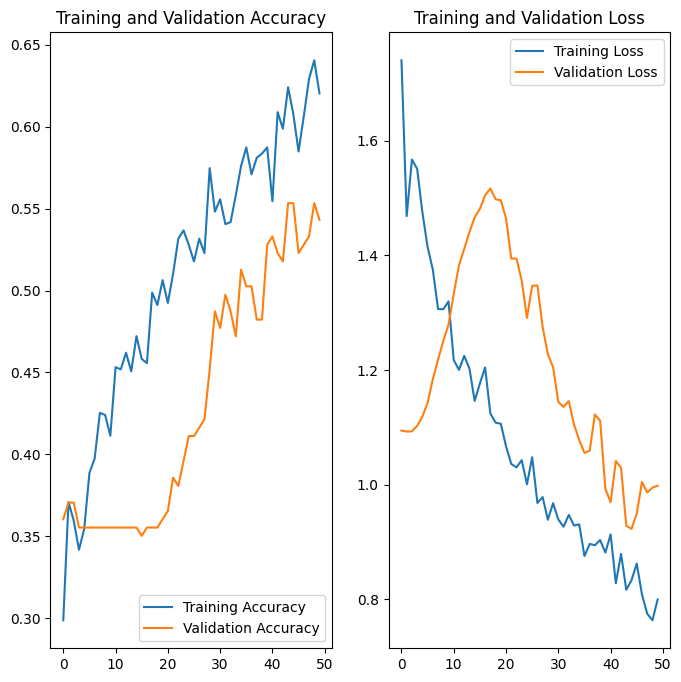
\includegraphics[width=\linewidth]{figures/without_preprocessing.png}
  \caption{No Preprocessing}
  \label{fig:no_preprocessing_plots}
\end{figure}

\begin{figure}[H]
  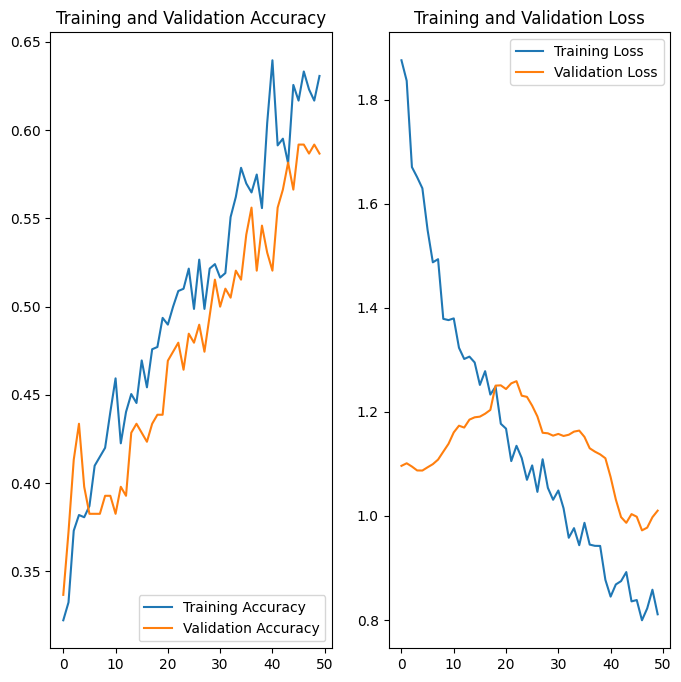
\includegraphics[width=\linewidth]{figures/training_validation_results.png}
  \caption{With Sobel Edge Detection only}
  \label{fig:sobel_edge_plots}
\end{figure}

\begin{figure}[H]
  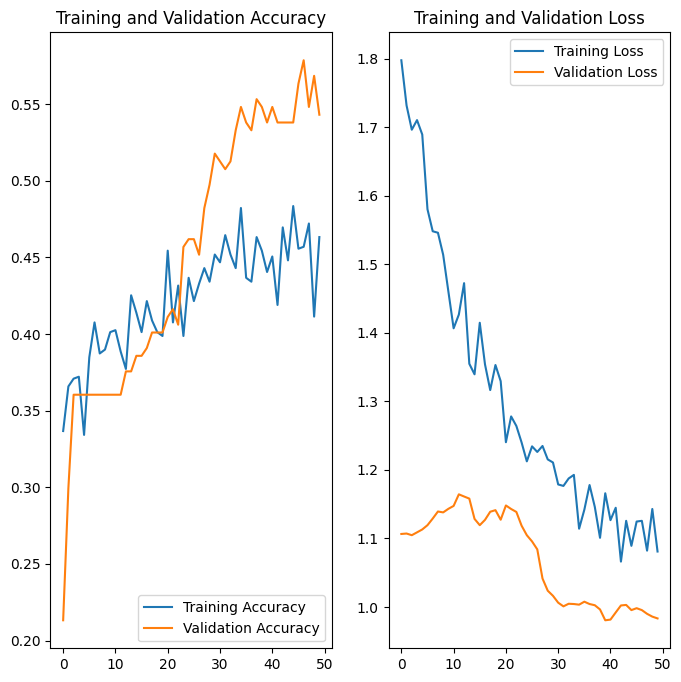
\includegraphics[width=\linewidth]{figures/with_data_aug.png}
  \caption{With Data Augmentation only}
  \label{fig:data_aug_plots}
\end{figure}

\begin{figure}[H]
  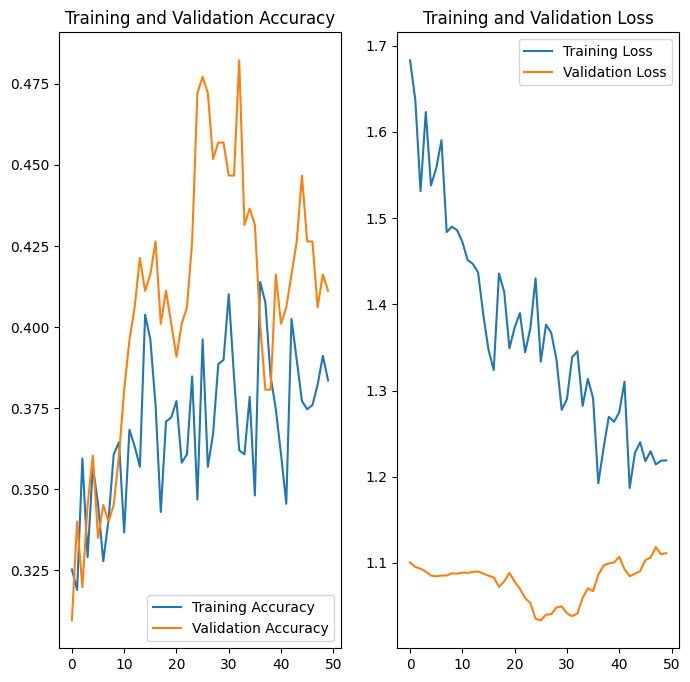
\includegraphics[width=\linewidth]{figures/with_data_aug_and_sobel_edge.png}
  \caption{With both Sobel Edge Detection and Data Augmentation}
  \label{fig:sobel_edge_and_data_aug_plots}
\end{figure}

The use of sobel edge detection help improved object detection and segmentation, notably improving hair boundary delineation in the images as seen in Figure~\ref{fig:sobel_edge_hairtypes}. Given our dataset only consists of 987 valid images, data augmentation was important in addressing the limited data situation. Despite its benefits, the best model performance was obseved with Sobel Edge Detection only, leading us to exlude data augmentation in next phases.

\subsection{Modeling}


% explain first the simple model. creating cnn model needs to find the balance between the appropriate amount of convolutional layers to be used and the complexity of the model. this is without dropout and batchnormalization

%  we commonly use relu for activation function but what if we use leakyrelu. mention the pros of leakyrelu and show the performance

%  using flatten only gives a very high training accuracy but at the expense of low validation accuracy. it always overfits so lets see the results

%  we also tried experimenting with using many convolutional layers and using globalaverage pooling only. let's see thje results of using globalaveragepooling and this complex layers

% discuss that there are scenarios that we can observe wherein the validation accuracy doesnt change in many epochs

% show the experiments that resulted to the creation of our model

